% !TEX program = xelatex
\documentclass[aspectratio=169,11pt]{beamer}

\usepackage[UTF8]{ctex}
\setCJKmainfont{SimSun}[BoldFont=SimHei,ItalicFont=KaiTi]
\setCJKsansfont{SimHei}

\usetheme{Madrid}
\usecolortheme{whale}
\setbeamertemplate{navigation symbols}{}
\setbeamertemplate{footline}[frame number]

\usepackage{xcolor}
\definecolor{mainblue}{HTML}{1565C0}
\definecolor{accentorg}{HTML}{FF6F00}
\definecolor{goodgreen}{HTML}{2E7D32}
\definecolor{badred}{HTML}{C62828}
\definecolor{purp}{HTML}{6A1B9A}
\definecolor{lightbg}{HTML}{F5F7FA}
\definecolor{graytext}{HTML}{757575}

\setbeamercolor{structure}{fg=mainblue}
\setbeamercolor{frametitle}{bg=mainblue,fg=white}
\setbeamercolor{title}{bg=mainblue!90,fg=white}
\setbeamercolor{block title}{bg=mainblue,fg=white}
\setbeamercolor{block body}{bg=lightbg}
\setbeamercolor{block title alerted}{bg=badred,fg=white}
\setbeamercolor{block body alerted}{bg=badred!5}
\setbeamercolor{block title example}{bg=goodgreen,fg=white}
\setbeamercolor{block body example}{bg=goodgreen!5}

\usepackage{tikz}
\usetikzlibrary{arrows.meta,positioning,calc,shapes.geometric,fit,backgrounds}
\usepackage{fontawesome5}
\usepackage{booktabs}
\usepackage{amsmath}

% 全部在preamble定义style，避免Beamer的#参数冲突
\tikzset{
  stepblue/.style={rectangle, rounded corners=6pt, draw=mainblue, fill=mainblue!10,
    minimum width=22mm, minimum height=22mm, align=center, font=\small},
  steporg/.style={rectangle, rounded corners=6pt, draw=accentorg, fill=accentorg!10,
    minimum width=22mm, minimum height=22mm, align=center, font=\small},
  steppurp/.style={rectangle, rounded corners=6pt, draw=purp, fill=purp!10,
    minimum width=22mm, minimum height=22mm, align=center, font=\small},
  stepgreen/.style={rectangle, rounded corners=6pt, draw=goodgreen, fill=goodgreen!10,
    minimum width=22mm, minimum height=22mm, align=center, font=\small},
  stepdark/.style={rectangle, rounded corners=6pt, draw=mainblue!80!black, fill=mainblue!5,
    minimum width=22mm, minimum height=22mm, align=center, font=\small},
  stepred/.style={rectangle, rounded corners=6pt, draw=badred!80, fill=badred!8,
    minimum width=32mm, minimum height=15mm, align=center, font=\small},
  boxblue/.style={rectangle, rounded corners=5pt, draw=mainblue, fill=mainblue!8,
    minimum width=32mm, minimum height=15mm, align=center, font=\small},
  boxred/.style={rectangle, rounded corners=5pt, draw=badred!80, fill=badred!8,
    minimum width=32mm, minimum height=15mm, align=center, font=\small},
  boxpurp/.style={rectangle, rounded corners=5pt, draw=purp, fill=purp!8,
    minimum width=32mm, minimum height=15mm, align=center, font=\small},
  boxgreen/.style={rectangle, rounded corners=5pt, draw=goodgreen, fill=goodgreen!8,
    minimum width=32mm, minimum height=15mm, align=center, font=\small},
  boxorg/.style={rectangle, rounded corners=5pt, draw=accentorg!80, fill=accentorg!8,
    minimum width=32mm, minimum height=15mm, align=center, font=\small},
  doneitem/.style={rectangle, rounded corners=4pt, fill=goodgreen!15, draw=goodgreen,
    minimum width=60mm, minimum height=9mm, font=\small, text=goodgreen!80!black, align=left},
  extraitem/.style={rectangle, rounded corners=4pt, fill=mainblue!15, draw=mainblue,
    minimum width=60mm, minimum height=9mm, font=\small, text=mainblue!80!black, align=left},
  kvblue/.style={rectangle, rounded corners=4pt, fill=mainblue!10, draw=mainblue!40,
    minimum width=50mm, minimum height=12mm, font=\small, align=left, inner xsep=6pt},
  kvorg/.style={rectangle, rounded corners=4pt, fill=accentorg!10, draw=accentorg!40,
    minimum width=50mm, minimum height=12mm, font=\small, align=left, inner xsep=6pt},
  kvpurp/.style={rectangle, rounded corners=4pt, fill=purp!10, draw=purp!40,
    minimum width=50mm, minimum height=12mm, font=\small, align=left, inner xsep=6pt},
  kvgreen/.style={rectangle, rounded corners=4pt, fill=goodgreen!10, draw=goodgreen!40,
    minimum width=50mm, minimum height=12mm, font=\small, align=left, inner xsep=6pt},
  phasegreen/.style={rectangle, rounded corners=5pt, fill=goodgreen!12, draw=goodgreen,
    minimum width=100mm, minimum height=16mm, font=\small, align=left, inner xsep=8pt},
  phaseblue/.style={rectangle, rounded corners=5pt, fill=mainblue!12, draw=mainblue,
    minimum width=100mm, minimum height=16mm, font=\small, align=left, inner xsep=8pt},
  phasepurp/.style={rectangle, rounded corners=5pt, fill=purp!12, draw=purp,
    minimum width=100mm, minimum height=16mm, font=\small, align=left, inner xsep=8pt},
}

\title{向量化存储 Pipeline v2.0}
\subtitle{动力装备知识图谱RAG系统 — 第一阶段进展汇报}
\author{纪文龙}
\date{2026年4月10日}
\institute{GitLab: \texttt{jiwenlong/vectorize-pipeline}}

\begin{document}

% SLIDE 1
\begin{frame}
\titlepage
\end{frame}

% SLIDE 2
\begin{frame}{任务完成情况}
\begin{center}
\begin{tikzpicture}
  \node[doneitem] (t0) at (0,0)   {\faCheckCircle\; 任务0：搭环境 \& 克隆仓库};
  \node[doneitem] (t1) at (0,-1.2) {\faCheckCircle\; 任务1：跑通现有Pipeline};
  \node[doneitem] (t2) at (0,-2.4) {\faCheckCircle\; 任务2：分析数据质量};
  \node[doneitem] (t3) at (0,-3.6) {\faCheckCircle\; 任务3：完成向量化存储};
  \node[doneitem] (t4) at (0,-4.8) {\faCheckCircle\; 任务4：组会汇报材料};

  \node[extraitem] (e1) at (7.5, 0) {\faStar\; 数据清洗（短文本合并）};
  \node[extraitem] (e2) at (7.5,-1.2) {\faStar\; BM25 混合检索};
  \node[extraitem] (e3) at (7.5,-2.4) {\faStar\; RRF 融合排序};
  \node[extraitem] (e4) at (7.5,-3.6) {\faStar\; 端到端 RAG 问答框架};
  \node[extraitem] (e5) at (7.5,-4.8) {\faStar\; 代码推送 GitLab};

  \node[font=\small\bfseries\color{goodgreen}, anchor=south] at (0,0.6) {指定任务（全部完成）};
  \node[font=\small\bfseries\color{mainblue}, anchor=south] at (7.5,0.6) {额外完成};
\end{tikzpicture}
\end{center}
\end{frame}

% SLIDE 3: Pipeline
\begin{frame}{Pipeline 全流程}
\begin{center}
\begin{tikzpicture}
  \node[stepblue] (s1) at (0,0) {\faFileCode\\[2pt] \textbf{解析JSON}\\[1pt] {\scriptsize 246块}};
  \node[steporg] (s15) at (2.8,0) {\faBroom\\[2pt] \textbf{数据清洗}\\[1pt] {\scriptsize 228块}};
  \node[steppurp] (s2) at (5.6,0) {\faCut\\[2pt] \textbf{文本分块}\\[1pt] {\scriptsize 16 chunk}};
  \node[stepgreen] (s3) at (8.4,0) {\faProjectDiagram\\[2pt] \textbf{BGE-m3}\\[1pt] {\scriptsize 1024维}};
  \node[stepdark] (s4) at (11.2,0) {\faDatabase\\[2pt] \textbf{Chroma}\\[1pt] {\scriptsize 持久化}};

  \draw[-{Stealth[length=4pt]},mainblue,line width=1.5pt] (s1) -- (s15);
  \draw[-{Stealth[length=4pt]},accentorg,line width=1.5pt] (s15) -- (s2);
  \draw[-{Stealth[length=4pt]},purp,line width=1.5pt] (s2) -- (s3);
  \draw[-{Stealth[length=4pt]},goodgreen,line width=1.5pt] (s3) -- (s4);

  \node[boxred] (s5) at (3.5,-3) {\faSearch\; \textbf{混合检索}\\[2pt]{\scriptsize 语义+BM25}};
  \node[boxorg] (s6) at (7.7,-3) {\faComments\; \textbf{RAG问答}\\[2pt]{\scriptsize 端到端}};

  \draw[-{Stealth[length=4pt]},mainblue!80!black,line width=1.5pt] (s4.south) -- ++(0,-0.8) -| (s5.north);
  \draw[-{Stealth[length=4pt]},badred,line width=1.5pt] (s5) -- (s6);

  \node[rectangle, rounded corners=4pt, draw=graytext, fill=white,
    font=\small\color{graytext}, align=center] (q) at (0.5,-3) {\faUser\; 用户查询};
  \draw[-{Stealth[length=3pt]}, graytext, dashed] (q) -- (s5);
\end{tikzpicture}
\end{center}
\end{frame}

% SLIDE 4: 数据概况
\begin{frame}{数据概况}
\begin{columns}[T]
\column{0.55\textwidth}
\begin{tikzpicture}
  \node[kvblue] (k1) at (0, 0)    {\textbf{文档数} \hfill 1 篇};
  \node[kvblue] (k2) at (0,-1.4)  {\textbf{总页数} \hfill 4 页};
  \node[kvorg] (k3) at (0,-2.8) {\textbf{标注块} \hfill 246 个};
  \node[kvpurp] (k4) at (0,-4.2)  {\textbf{清洗后} \hfill 228 个};
  \node[kvgreen] (k5) at (0,-5.6) {\textbf{Chunk数} \hfill 16 个};
\end{tikzpicture}

\column{0.45\textwidth}
\textbf{标签分布}

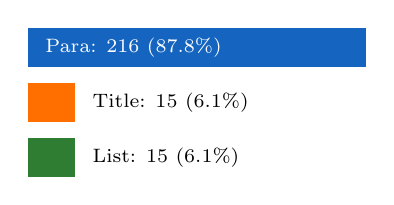
\begin{tikzpicture}
  \fill[mainblue] (0,0) rectangle (4.3,0.5);
  \node[font=\scriptsize\color{white}, anchor=west] at (0.1,0.25) {Para: 216 (87.8\%)};
  \fill[accentorg] (0,-0.7) rectangle (0.6,-0.2);
  \node[font=\scriptsize, anchor=west] at (0.7,-0.45) {Title: 15 (6.1\%)};
  \fill[goodgreen] (0,-1.4) rectangle (0.6,-0.9);
  \node[font=\scriptsize, anchor=west] at (0.7,-1.15) {List: 15 (6.1\%)};
\end{tikzpicture}

\vspace{6mm}
\textbf{Chunk 统计}

\begin{tabular}{ll}
平均长度 & 429 字符 \\
最短/最长 & 248 / 498 字符 \\
向量维度 & 1024 \\
\end{tabular}
\end{columns}
\end{frame}

% SLIDE 5: 数据质量
\begin{frame}{数据质量分析与修复}
\begin{columns}[T]
\column{0.48\textwidth}
\begin{alertblock}{问题1：OCR碎片}
标注时bbox切割过细，产生碎片：

\smallskip
{\small
\texttt{"程体系。"} \texttt{"建方法"} \texttt{"印证。"}
}
\end{alertblock}

\begin{exampleblock}{修复：短文本合并}
\texttt{clean\_blocks()}: 不足10字符自动合并

\smallskip
\centering
246块 $\xrightarrow{\text{合并18个}}$ 228块 \quad {\color{goodgreen}\faCheckCircle}
\end{exampleblock}

\column{0.48\textwidth}
\begin{alertblock}{问题2：双栏交叉（待解决）}
PDF左右栏纵坐标重叠，文字交叉

\smallskip
{\small 左栏3行 $\to$ 右栏1行 $\to$ 左栏4行}
\end{alertblock}

\begin{block}{反问题材}
需要在JSON中获取\textbf{x坐标}：
\begin{itemize}\small
  \item $x < 50\%$：左栏
  \item $x \geq 50\%$：右栏
  \item 每栏内按y排序
\end{itemize}
\end{block}
\end{columns}
\end{frame}

% SLIDE 6: Title分块
\begin{frame}{分块策略：Title 触发新 Chunk}
\begin{columns}[T]
\column{0.48\textwidth}
\begin{alertblock}{\faTimesCircle\; 普通分块}
\begin{tikzpicture}[font=\scriptsize]
  \node[rectangle, draw=badred!50, fill=badred!5, rounded corners=3pt,
    text width=50mm, inner sep=4pt, align=left] at (0,0) {
    {\color{graytext} ...正文正文正文...}\\[1pt]
    {\color{badred}\bfseries 一、新章节标题}\\[1pt]
    {\color{graytext} $\uparrow$ 标题粘在上段末尾}
  };
  \node[rectangle, draw=gray!30, fill=gray!5, rounded corners=3pt,
    text width=50mm, inner sep=4pt, align=left] at (0,-1.6) {
    {\color{graytext} 新章节正文...}\\[1pt]
    {\color{graytext} $\uparrow$ 新chunk没标题}
  };
\end{tikzpicture}
\end{alertblock}

\column{0.48\textwidth}
\begin{exampleblock}{\faCheckCircle\; 我的分块}
\begin{tikzpicture}[font=\scriptsize]
  \node[rectangle, draw=gray!30, fill=gray!5, rounded corners=3pt,
    text width=50mm, inner sep=4pt, align=left] at (0,0) {
    {\color{graytext} ...正文正文正文...}\\[1pt]
    {\color{graytext} $\uparrow$ 上一段完整结束}
  };
  \node[rectangle, draw=goodgreen!50, fill=goodgreen!5, rounded corners=3pt,
    text width=50mm, inner sep=4pt, align=left] at (0,-1.6) {
    {\color{goodgreen}\bfseries 一、新章节标题}\\[1pt]
    {\color{graytext} 新章节正文...}\\[1pt]
    {\color{graytext} $\uparrow$ 标题+正文同一chunk}
  };
\end{tikzpicture}
\end{exampleblock}
\end{columns}
\end{frame}

% SLIDE 7: 混合检索
\begin{frame}{混合检索：语义 + BM25 + RRF}
\begin{columns}[T]
\column{0.32\textwidth}
\begin{block}{\faProjectDiagram\; 语义检索}
BGE-m3, 1024维

\smallskip
{\small
\textbf{优}: 理解同义词\\
\textbf{弱}: 精确关键词差
}
\end{block}

\column{0.32\textwidth}
\begin{block}{\faSearch\; BM25关键词}
jieba分词 + TF-IDF

\smallskip
{\small
\textbf{优}: 精确匹配\\
\textbf{弱}: 不懂同义词
}
\end{block}

\column{0.32\textwidth}
\begin{exampleblock}{\faMagic\; RRF融合}
$\alpha{=}0.7$ 语义

$(1{-}\alpha){=}0.3$ BM25

两路互补
\end{exampleblock}
\end{columns}

\vspace{3mm}
\begin{center}
\begin{tabular}{lccc}
\toprule
\textbf{查询} & \textbf{语义} & \textbf{BM25} & \textbf{哪个更好} \\
\midrule
"燃气轮机健康管理" & 0.685 & 3.2 & 都行 \\
"布鲁姆认知过程" & {\color{badred}0.387} & {\color{goodgreen}\textbf{4.7}} & BM25胜 \\
"船舶动力装置" & {\color{goodgreen}\textbf{0.542}} & {\color{badred}0.0} & 语义胜 \\
\bottomrule
\end{tabular}
\end{center}
\end{frame}

% SLIDE 8: RAG
\begin{frame}{端到端 RAG 问答}
\begin{center}
\begin{tikzpicture}
  \node[boxblue] (q) at (0,0) {\faUser\; \textbf{用户提问}\\[2pt]{\scriptsize "知识体系如何构建？"}};
  \node[boxred] (r) at (4.5,0) {\faSearch\; \textbf{混合检索}\\[2pt]{\scriptsize Top-3 段落}};
  \node[boxpurp] (c) at (9,0) {\faLayerGroup\; \textbf{拼接上下文}\\[2pt]{\scriptsize 来源+页码+原文}};
  \node[boxgreen] (a) at (13,0) {\faRobot\; \textbf{生成答案}\\[2pt]{\scriptsize 智谱/千问API}};

  \draw[-{Stealth[length=4pt]},mainblue,line width=1.2pt] (q) -- (r);
  \draw[-{Stealth[length=4pt]},badred,line width=1.2pt] (r) -- (c);
  \draw[-{Stealth[length=4pt]},purp,line width=1.2pt] (c) -- (a);

  \node[font=\scriptsize\bfseries\color{goodgreen}] at (2.25, -1.3) {\faCheckCircle\; 已完成};
  \node[font=\scriptsize\bfseries\color{goodgreen}] at (6.75, -1.3) {\faCheckCircle\; 已完成};
  \node[font=\scriptsize\bfseries\color{goodgreen}] at (11, -1.3) {\faCheckCircle\; 框架就绪};
  \node[font=\scriptsize\bfseries\color{accentorg}] at (13, -1.3) {\faClock\; 待接入};
\end{tikzpicture}
\end{center}

\vspace{4mm}
\begin{columns}[T]
\column{0.55\textwidth}
\begin{block}{当前能力}
\begin{itemize}
  \item 问题 $\to$ 混合检索Top-3段落
  \item 自动标注来源页码和相关度
  \item 展示原文片段供参考
\end{itemize}
\end{block}

\column{0.42\textwidth}
\begin{block}{运行方式}
{\ttfamily\scriptsize
python 向量化存储.py\\
~~--vectorize\\
~~--ask "你的问题"
}
\end{block}
\end{columns}
\end{frame}

% SLIDE 9: 下一步
\begin{frame}{下一步计划}
\begin{center}
\begin{tikzpicture}
  \node[phasegreen] (p1) at (0, 0) {
    {\bfseries\color{goodgreen}\faCheckCircle\; 本周（已完成）}\hfill
    {\scriptsize Pipeline + 数据分析 + 混合检索 + GitLab}
  };
  \node[phaseblue] (p2) at (0, -2) {
    {\bfseries\color{mainblue}\faArrowCircleRight\; 2-4周内}\hfill
    {\scriptsize 全量1000本手册 / 接入LLM API / Web演示}
  };
  \node[phasepurp] (p3) at (0, -4) {
    {\bfseries\color{purp}\faFlask\; 暑假前}\hfill
    {\scriptsize Graph RAG / 知识图谱 / SCI论文（6-7月）}
  };

  \draw[-{Stealth[length=4pt]}, goodgreen, line width=1.5pt] (p1.south) -- (p2.north);
  \draw[-{Stealth[length=4pt]}, mainblue, line width=1.5pt] (p2.south) -- (p3.north);
\end{tikzpicture}
\end{center}
\end{frame}

% SLIDE 10: 谢谢
\begin{frame}{}
\begin{center}
\vspace{15mm}
{\Huge\bfseries\color{mainblue} 谢谢，请指导}

\vspace{10mm}
{\large\color{graytext}
\faGitlab\; \texttt{jiwenlong/vectorize-pipeline}\\[6pt]
\faCodeBranch\; 2次提交 \quad \faPython\; 400+ 行代码
}
\end{center}
\end{frame}

\end{document}
